\subsection{Physical validation}
We also tested the planner and controller on our physical F1/10 car.
%
This is to show the practicality of our simple map-less planning and control in the presence of noise, unstructured environment, and limited computational resource.
%
For example, Hokuyo UST-10LX LiDAR provides a new point-cloud every 25 milliseconds, but our planning and control is an order of magnitude faster on the Nvidia Jetson TX2's CPU so we can process every point cloud.
%
We tested the car in two tracks.
%
The simpler one is shown in Fig.~\ref{fig:physical_track} where the track boundaries is mostly structured using corrugated cardboard rolls.
%
The harder track (provided in the videos) is an office with chairs and tables around the office walls and in the middle of the office.
%
Our algorithm manages to successfully complete a lap while avoiding obstacles on both of these tracks.

\begin{figure}[!t]
\centering
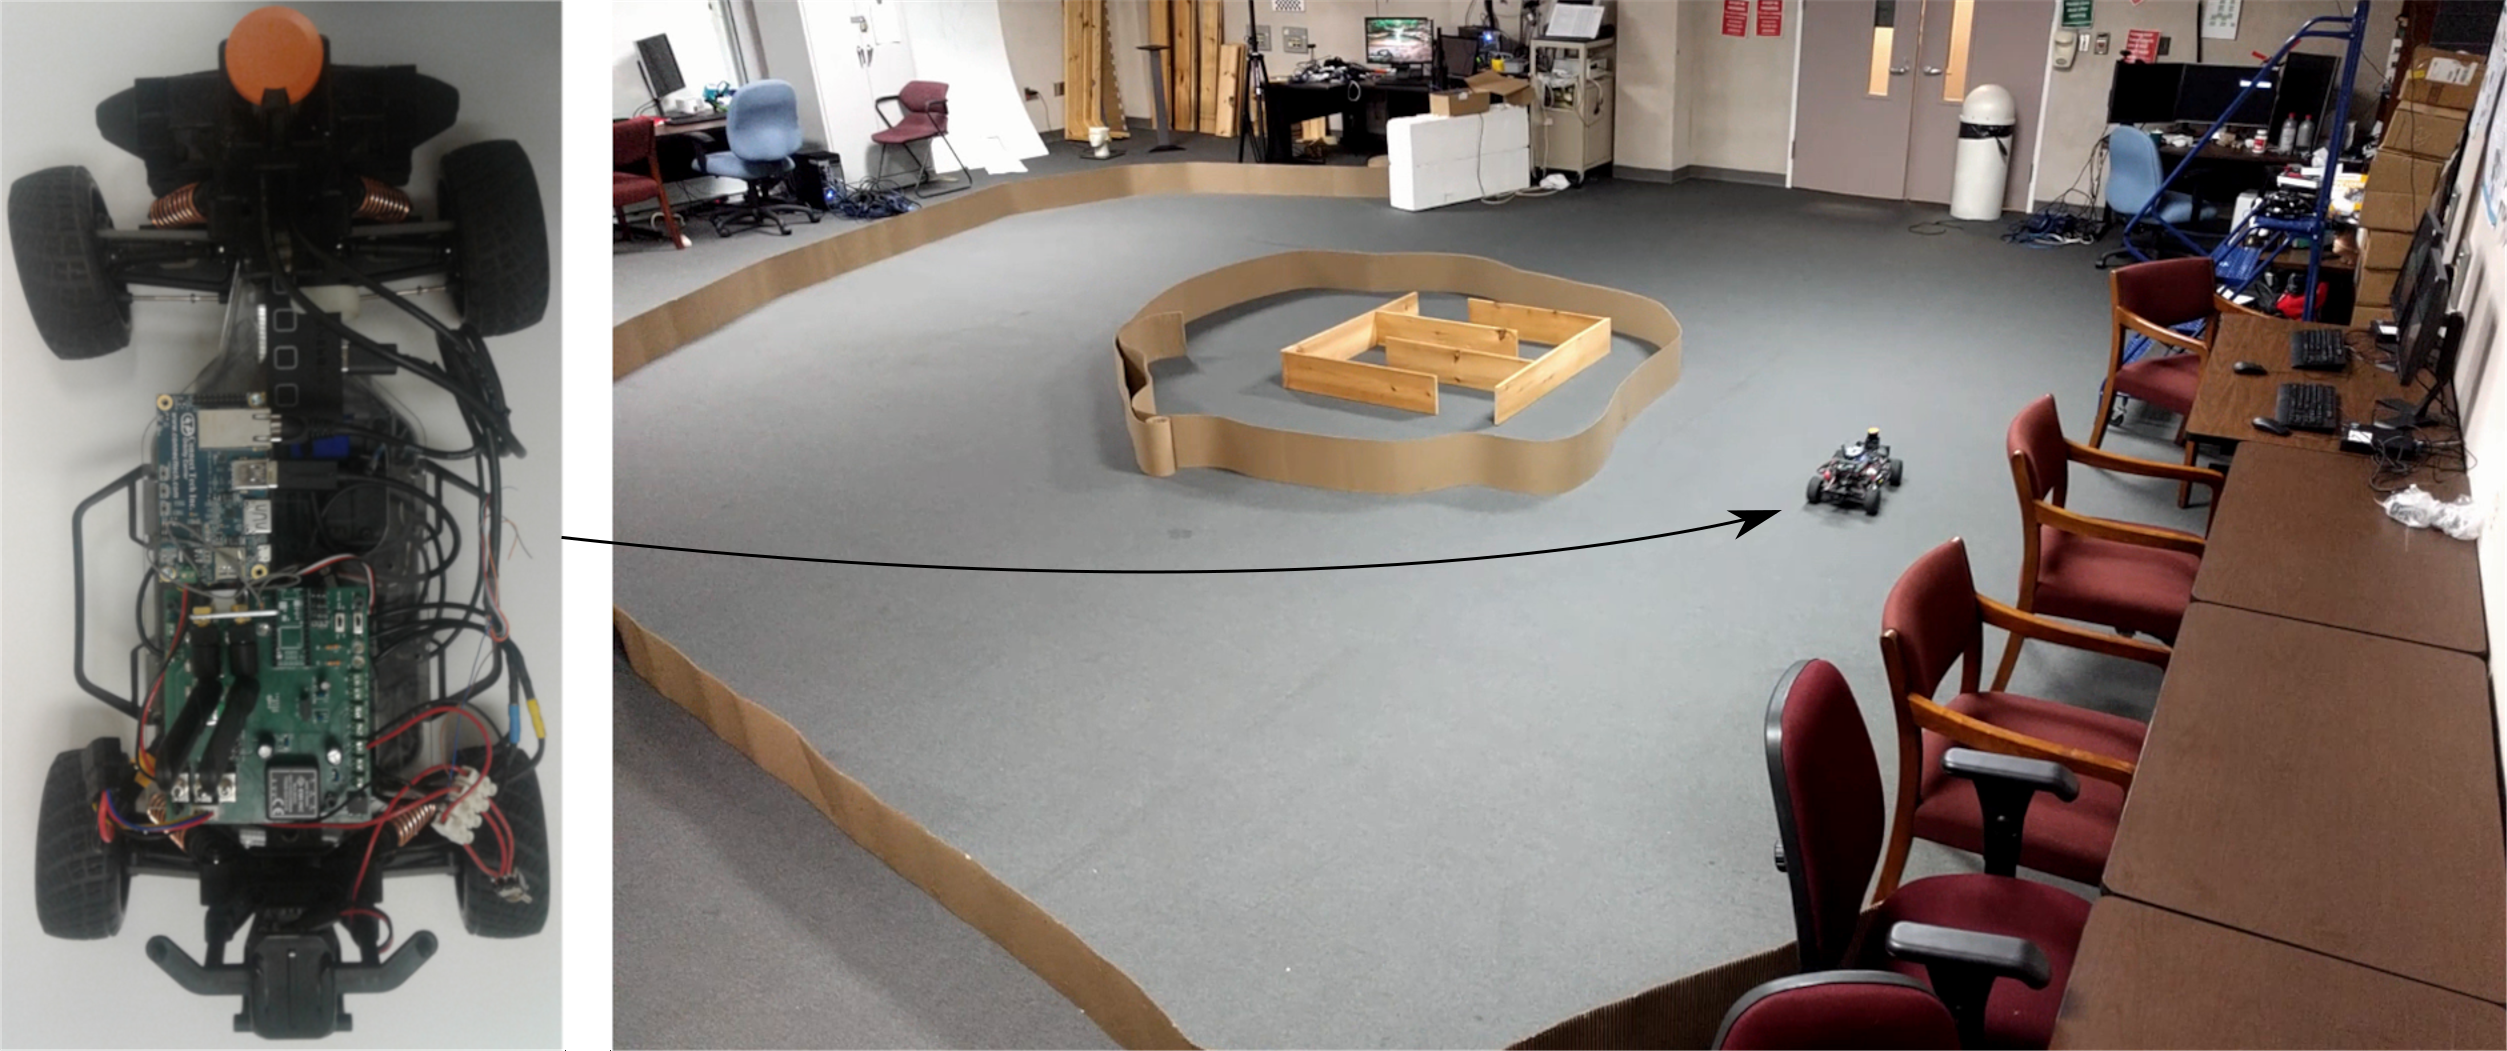
\includegraphics[width=85mm]{Figures/physical_track.png}
\caption{Physical validations.}
\label{fig:physical_track}
\end{figure}


